% =====================================================================
%  Pricing the DeFi Tail -- CBT 2026 conference talk.
%
%  Venue : 10th International Workshop on Cryptocurrencies and
%          Blockchain Technology (CBT 2026), co-located with
%          ESORICS 2026, Rome, Thursday 17 September 2026.
%  Slot  : "DECENTRALIZED FINANCE" session, 10:30-12:30 CEST, 5 papers
%          -> 24 min per paper including hand-over and questions.
%  Built for 20 minutes of speaking + ~4 minutes of questions.
%
%  Timing plan (target minutes, cumulative):
%    Motivation & question .............. 3   (slides 2-4)
%    Data ............................... 4   (slides 5-7)
%    Method ............................. 3   (slides 8-9)
%    The tail ........................... 5   (slides 10-13)
%    Who bears it ....................... 4   (slides 14-16)
%    Policy & close ..................... 1   (slides 17-18)
%
%  Compile:  make            (or: pdflatex slides.tex twice)
% =====================================================================
\documentclass[10pt,xcolor=x11names,aspectratio=169]{beamer}
\usepackage{zhaw-theme}
% =====================================================================
%  presentation-info.tex  --  shared metadata for the CBT 2026 deck.
% =====================================================================
\newcommand{\zhawcoursetitle}{Pricing the DeFi Tail}
\renewcommand{\zhawinstitute}{ZHAW School of Engineering}
% Footer parts, in the order the corporate design prescribes:
%   ZHAW School of Engineering | Organisational unit | Document name
\renewcommand{\zhawunit}{IDS Institute for Data Science}
\newcommand{\zhawdocname}{\zhawcoursetitle}

\renewcommand{\zhawpresenter}{Nils Bundi}

% Details for the closing slide (\closingslide).
\renewcommand{\zhawposition}{Senior Lecturer}
\renewcommand{\zhawaddress}{Technikumstrasse 81\\8400 Winterthur, Switzerland}
\renewcommand{\zhawphone}{+41 58 934 71 71}
\renewcommand{\zhawemail}{bund@zhaw.ch}
\renewcommand{\zhawweb}{www.zhaw.ch/engineering}

% Standard title-page block.
\author{\zhawpresenter}
\institute{\zhawinstitute}
\date{CBT 2026 \textbar\ Rome, 17 September 2026}

% Default footer (left cell); middle cell is free for \mfooter{...},
% right cell holds the frame number.
% The full corporate-design line (school | unit | document) wraps at this slide
% width, so the left cell carries the short paper title alone; school and unit
% are still set above for the title and closing slides.
\lfooter{\zhawdocname}


\usepackage{booktabs}

\newcommand{\VaR}{\operatorname{VaR}}
\newcommand{\E}{\mathbb{E}}
\newcommand{\NB}{\mathrm{NB}}
\newcommand{\bps}{\,bps}

\mfooter{CBT 2026 \textbar\ Rome}
% Title page: the full paper title rides the seam in the 'Sky' connector box,
% the venue sits under it (workshop line bold, series name below), then author
% and the place/date line.
\title{Pricing the DeFi Tail:\\
Do Protocols or Depositors\\
Price Operational Risk?}
\subtitle{\textbf{CBT 2026 --- 10th International Workshop on}\\[0.5mm]
{\normalsize Cryptocurrencies and Blockchain Technology}}

\begin{document}

% ---------------------------------------------------------------- title
\begin{frame}[plain,noframenumbering]\titlepage\end{frame}

% =====================================================================
\section{The question}
% =====================================================================

% Opening slide: four headline screenshots, captured from the publishers' own
% pages (see figures/headlines/). Every one of the four is a row of
% ../data/events_consolidated.csv.
\begin{frame}{The losses are real, and they are recent}
  \vskip -3mm
  \begin{center}
  \setlength{\tabcolsep}{2.5mm}\renewcommand{\arraystretch}{1.0}
  \begin{tabular}{@{}cc@{}}
    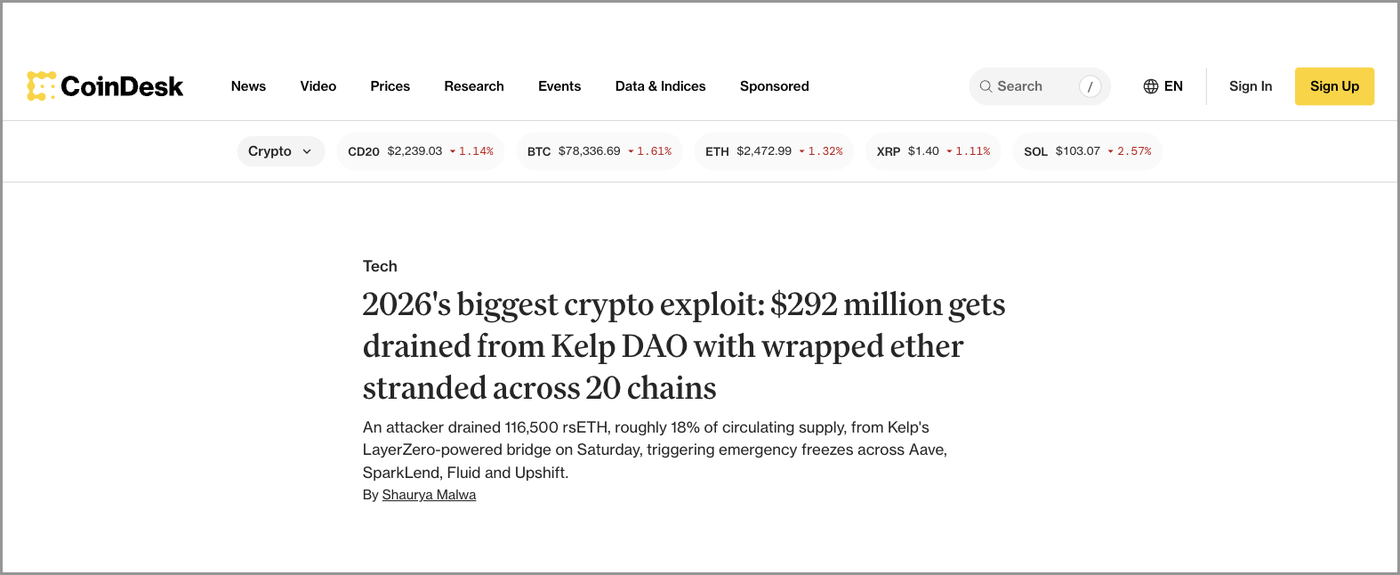
\includegraphics[width=0.435\linewidth]{figures/headlines/kelp} &
    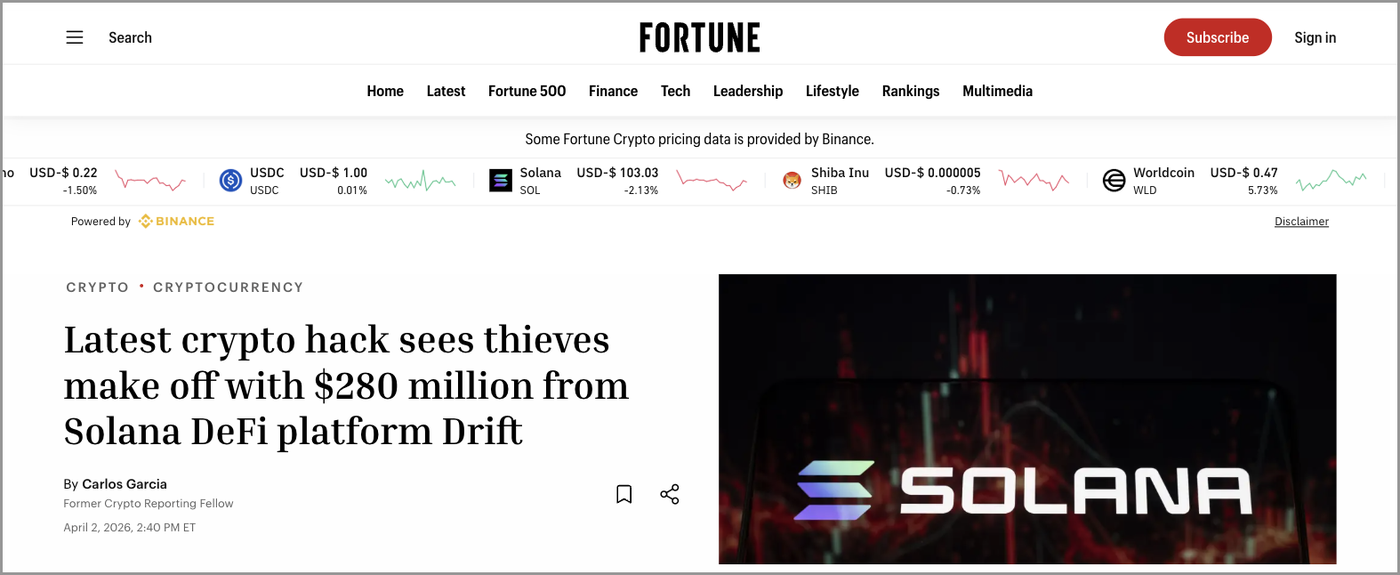
\includegraphics[width=0.435\linewidth]{figures/headlines/drift} \\[0.4mm]
    {\scriptsize\hl{USD 292\,m}, Bridge --- a forged cross-chain message} &
    {\scriptsize\hl{USD 290\,m}, Derivatives --- admin approvals abused} \\[1.2mm]
    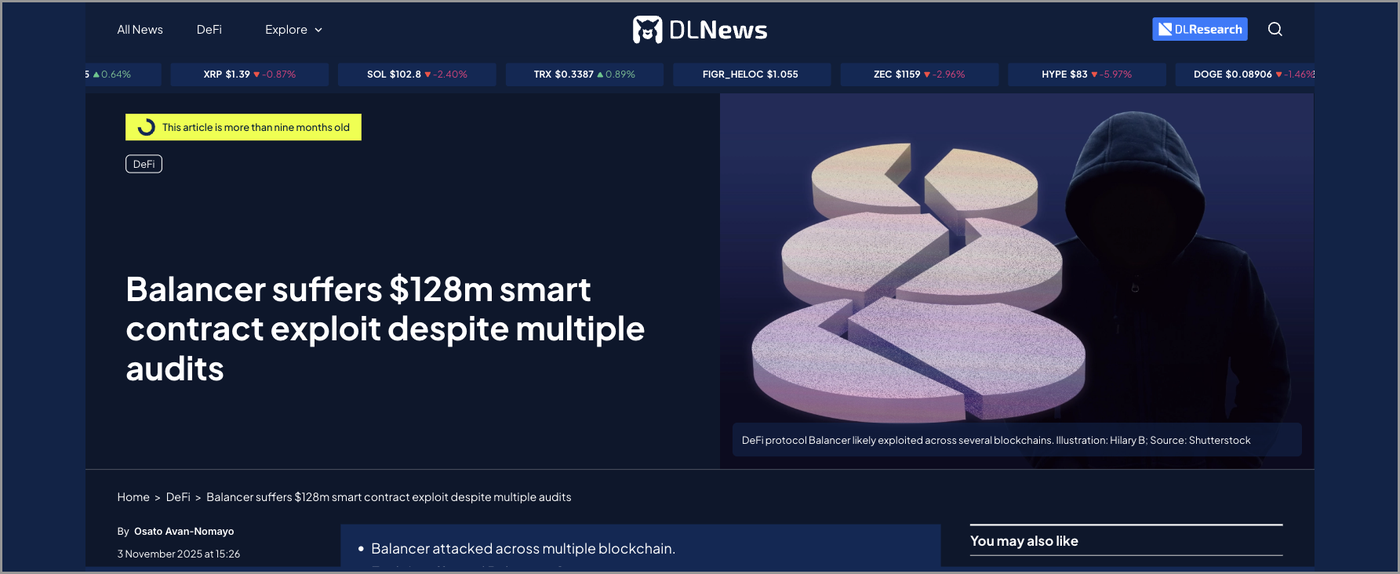
\includegraphics[width=0.435\linewidth]{figures/headlines/balancer} &
    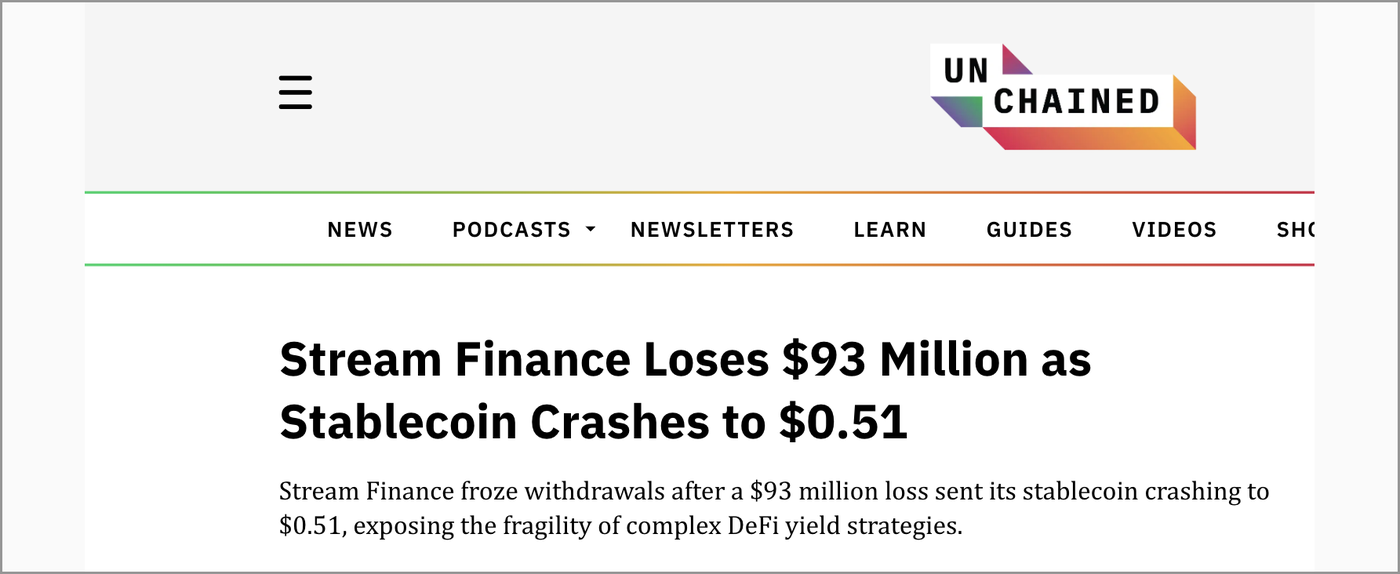
\includegraphics[width=0.435\linewidth]{figures/headlines/stream} \\[0.4mm]
    {\scriptsize\hl{USD 128\,m}, DEX --- a rounding error, after audits} &
    {\scriptsize\hl{USD 93\,m}, Yield --- no exploit at all} \\
  \end{tabular}
  \end{center}
\end{frame}

\begin{frame}{DeFi removes many risks --- operational risk is not one of them}
  DeFi's architecture genuinely removes several bank-balance-sheet risks:
  smart-contract custody replaces the custodian, settlement is atomic,
  counterparty credit risk collapses into overcollateralization.
  \begin{itemize}
    \item \hl{Operational risk remains} --- losses from failed processes,
          people, systems and external events --- and in some cases
          concentrates: contract code, admin keys, oracles, economic design.
    \item Unlike a bank, DeFi is \hl{infrastructure}: no regulatory capital
          requirement, no deposit insurance, no resolution authority. Nothing
          stands between a loss and the depositor's claim unless a protocol
          chooses to put it there.
    \item Yet DeFi markets \hl{earn products} --- lending supply, yield vaults,
          stablecoin positions, crypto neobanks, etc.
  \end{itemize}
  \begin{takeaway}[The decisive difference]
    Not whether the risk exists --- it does, and it is measurable --- but
    \emph{who bears it} and \emph{whether anyone priced it}.
  \end{takeaway}
\end{frame}

\begin{frame}{Two responses, neither disciplined by a regulator}
  \begin{columns}[T]
    \begin{column}{0.48\textwidth}
      \textbf{The protocol can hold a buffer.}\\[2pt]
      Aave's Umbrella safety module, the Sky surplus buffer, Compound's
      reserve factor --- governance-owned reserves with the function Basel
      calls capital, sized by vote rather than by any loss model.
    \end{column}
    \begin{column}{0.48\textwidth}
      \textbf{Or the depositor demands a premium.}\\[2pt]
      A supply yield above the risk-free rate compensates the depositor for
      bearing the tail --- the market-discipline mechanism by which uninsured
      bank creditors price institutional risk.
    \end{column}
  \end{columns}
  \vskip 4mm
  The two are \hl{substitutes} for the same risk, chosen by different
  participants.
  \begin{block}{Research question}
    Is either response sized to the operational-risk tail it is meant to
    cover? Answering it needs a common benchmark --- so I first have to
    quantify the tail.
  \end{block}
\end{frame}

\begin{frame}{Contributions}
  \begin{enumerate}
    \item A \hl{consolidated event dataset}: seven public feeds, deduplicated,
          filtered to depositor-facing DeFi losses, tagged by sector and Basel
          Level-1 event type --- $n=1{,}075$, USD~$9.45$~B, 2020--2026.
    \item A \hl{per-sector Basel LDA}, fitted as a bank supervisor would, and
          benchmarked against banking operational risk.
    \item Both margins tested against that one benchmark: \hl{protocol capital
          buffers} and \hl{depositor risk premia}.
    \item Evidence that the two \hl{substitute} --- in the right direction, at
          the wrong order of magnitude --- and the policy that follows.
  \end{enumerate}
  \begin{takeaway}[Headline]
    The four buffered top-10 Lending venues cover $\sim 5\%$ of their modeled
    $\VaR_{99.9}$; unbuffered venues pay $+54$~bps against a tail worth
    $34$--$81\%$ of TVL.
  \end{takeaway}
\end{frame}

% =====================================================================
\section{Data}
% =====================================================================

\begin{frame}{Seven feeds, one deduplicated dataset}
  \begin{columns}[T]
    \begin{column}{0.53\textwidth}
      \footnotesize
      \begin{tabular}{l r r}
        \toprule
        Source & Raw & In dataset \\
        \midrule
        DefiLlama hack ledger      &   528 & 379 \\
        kismp123 DSI corpus        &   823 & 290 \\
        BlockSec Incidents Library &   285 & 201 \\
        rekt.news leaderboard      &   281 & 219 \\
        DeFiHackLabs catalog       &   615 & 163 \\
        de.fi/rekt-database        & 4{,}030 & 704 \\
        SlowMist Hacked            & 2{,}100 & 639 \\
        \midrule
        Consolidated (dedup.)      &       & 1{,}164 \\
        \bottomrule
      \end{tabular}
    \end{column}
    \begin{column}{0.43\textwidth}
      \small
      \begin{itemize}
        \item Median-across-sources loss reconciliation.
        \item Two-pass dedup: name within $\pm14$~d, then date $\pm7$~d and
              loss within $\pm10\%$.
        \item Out-of-scope removed (CEX, memecoins, NFTs, phishing): 153 events.
        \item A \hl{depositor-facing filter} drops 89 events (USD~$0.84$~B)
              whose loss the earn user does not bear.
        \item Working sample \hl{$n = 1{,}075$}, USD~$9.45$~B;
              $50\%$ cross-source confirmed.
      \end{itemize}
    \end{column}
  \end{columns}
  \begin{takeaway}[Why it matters]
    Prior work relies on a single feed, yet tail estimates are driven by the
    largest handful of events.
  \end{takeaway}
\end{frame}

\begin{frame}{Tagged to the banking taxonomy}
  Every event carries a DeFi sub-sector and a \hl{Basel Level-1 event type}
  --- textual evidence first, feed classification as fallback.
  \vskip 2mm
  \footnotesize
  \begin{tabular}{l p{2.9cm} p{7.2cm}}
    \toprule
    Code & Basel Level-1 & DeFi operational reading \\
    \midrule
    IF   & Internal Fraud & Rugpull, owner-drain, insider exit-scam, upgradeable-contract abuse. \\
    EF   & External Fraud & Contract bugs (reentrancy, access control), key compromise, DNS hijack. \\
    CPBP & Clients, Products, Business Practices & Economic-design attacks: flashloan governance, oracle and price manipulation. \\
    BDSF & Business Disruption, System Failures & Chain-level: MEV, sequencer outage, consensus issue, chain halt. \\
    EDPM & Execution, Delivery, Process Mgmt & Team-side configuration and deployment errors. \\
    \bottomrule
  \end{tabular}
  \normalsize
  \vskip 2mm
  EPWS and DPA have no on-chain analogue and are omitted. Seven sectors:
  Bridge, Lending, DEX, Yield, Stablecoin, Derivatives, Other.
\end{frame}

\begin{frame}{Sector and event type are orthogonal}
  \begin{columns}[T]
    \begin{column}{0.55\textwidth}
      \footnotesize\setlength{\tabcolsep}{3pt}
      Aggregate gross loss, USD~m
      \begin{tabular}{l r r r r r r}
        \toprule
        Sector & EF & IF & CPBP & EDPM & BDSF & Total \\
        \midrule
        Bridge      & 3{,}084 &  127 &   6 &  8 &  12 & 3{,}237 \\
        Lending     &    704 &  568 & 928 & 14 &   8 & 2{,}222 \\
        Stablecoin  &    178 &  105 & 456 & 27 &   8 &   773 \\
        Yield       &    430 &  267 & 206 & 17 &   6 &   926 \\
        DEX         & 1{,}044 &  136 & 221 &  0 &   1 & 1{,}402 \\
        Derivatives &    148 &    0 & 275 &  2 & 380 &   805 \\
        Other       &     35 &    4 &  48 &  0 &   0 &    87 \\
        \midrule
        Total & 5{,}623 & 1{,}207 & 2{,}140 & 68 & 415 & 9{,}452 \\
        \bottomrule
      \end{tabular}
    \end{column}
    \begin{column}{0.41\textwidth}
      \small
      \begin{itemize}
        \item Bridge and DEX are near-pure \hl{EF} --- code failing over pooled
              collateral. Bridge$\times$EF alone is $33\%$ of all losses.
        \item Lending and Stablecoin are \hl{CPBP}-heavy --- economic design,
              not code.
        \item Derivatives is the only sector with material \hl{BDSF}.
      \end{itemize}
      \vskip 2mm
      Aggregate mean loss USD~$8.79$~m, median USD~$0.50$~m,
      max USD~$624$~m (Ronin).
    \end{column}
  \end{columns}
  \begin{pitfall}[Consequence for the model]
    Sector totals span two orders of magnitude and the loss mechanism differs
    by sector, so a single pooled fit would be meaningless. Everything is
    fitted \hl{per sector}.
  \end{pitfall}
\end{frame}

% Slide-sized redraw of the paper's Fig. 1 (make_slide_figures.py): wide, with
% upright sector labels instead of the LNCS column's rotated ones.
\begin{frame}{Loss distributions differ sharply across sectors}
  \vskip -1mm
  \centering
  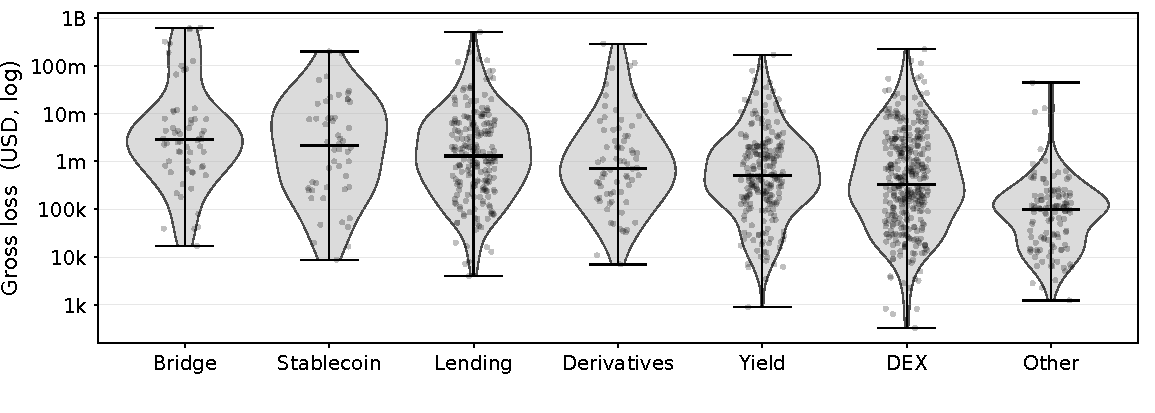
\includegraphics[width=\linewidth]{figures/violin_slide}\\[1.5mm]
  {\scriptsize Violins encode density, bars the median. Bridge carries the
  highest median event loss (USD~2.90~m) from the pooled collateral bridges
  hold.\par}
\end{frame}

% =====================================================================
\section{Method}
% =====================================================================

\begin{frame}{The loss-distribution approach, per sector}
  \begin{columns}[T]
    \begin{column}{0.48\textwidth}
      \textbf{Severity} --- peaks-over-threshold GPD on excesses
      $Y_i = X_i - u \mid X_i > u$:
      \[
        g_{\xi,\beta}(y) = \tfrac{1}{\beta}\bigl(1+\xi\tfrac{y}{\beta}\bigr)^{-(1/\xi+1)}
      \]
      Threshold $q^*$ by \hl{plateau stability} ($\hat\xi$ stable to
      $\tau=0.30$), subject to $n_u \ge 20$ and $n_u/n \ge 10\%$. The severity
      $F_X$ is then piecewise: the \hl{empirical body} below $u^*$, the
      \hl{GPD tail} above it.
      \vskip 3mm
      \textbf{Frequency} --- monthly negative binomial
      $N_s \sim \NB(\mu_s,\alpha_s)$; annual counts as twelve iid monthly
      draws.
    \end{column}
    \begin{column}{0.48\textwidth}
      \textbf{Compound aggregation}
      \[
        S_{\text{year}} = \sum_{i=1}^{N} X_i,
        \quad N \sim \NB(\hat\lambda,\hat\alpha),
        \quad X_i \overset{\text{iid}}{\sim} F_X
      \]
      $2\times 10^{5}$ simulated years per sector, each event capped at the
      largest single-protocol exposure.
      \vskip 2mm
      $\E[S]$ is the actuarial \hl{pure premium};
      $\VaR_{99.9}$ is the \hl{capital buffer} the Basel AMA would compute.
      Both expressed as a share of trailing-365d \hl{TVL} --- the on-chain
      analogue of assets on books.
    \end{column}
  \end{columns}
\end{frame}

\begin{frame}{From sector to protocol}
  No single protocol records enough events for its own fit --- the same
  problem Basel solves for data-poor banks with a business-line severity
  allocated by an exposure indicator.
  \begin{itemize}
    \item Fit once per sector; treat its protocols as sharing that loss
          process \hl{per unit of TVL} (credibility-theory shrinkage).
    \item A sector event strikes protocol $p$ with probability
          $\text{TVL}_p/\text{TVL}_s$, so
          $\lambda_p = (\text{TVL}_p/\text{TVL}_s)\,\lambda_s$, same severity,
          capped at $p$'s own exposure.
    \item The tail does \emph{not} thin linearly: with the single-loss
          approximation
          $\VaR_{99.9}(S_p)\approx F_X^{-1}(1-0.001/\lambda_p)$ scaling as
          $\text{TVL}_p^{\hat\xi}$, $\hat\xi<1$, the \hl{VaR-to-TVL ratio
          rises as a venue shrinks}.
  \end{itemize}
  \begin{pitfall}[So do not scale the sector ratio]
    Simulating $\VaR_{99.9}$ per venue rather than scaling the sector figure
    is what keeps the smaller venues from being understated.
  \end{pitfall}
\end{frame}

% =====================================================================
\section{The tail}
% =====================================================================

\begin{frame}{Severity: four sectors like a bank, three like cyber}
  \footnotesize
  \begin{center}
  \begin{tabular}{lrrrlrrr}
    \toprule
    Sector & $n$ & $q^*$ & $n_u$ & $\hat\xi$ \,[95\% CI] & $\hat\beta$ (USD m) & $V$ & $p$ \\
    \midrule
    Bridge      &  61 & 0.65 & 20 & $+1.87$ \,[$+0.58$, $+3.18$] & 17.6 & $-1.37$ & 0.17 \\
    Lending     & 207 & 0.90 & 21 & $+0.75$ \,[$-0.28$, $+1.50$] & 24.8 & $-1.32$ & 0.19 \\
    Stablecoin  &  52 & 0.60 & 21 & $+0.65$ \,[$-0.39$, $+1.33$] & 13.2 & $-0.03$ & 0.97 \\
    Derivatives &  71 & 0.65 & 25 & $+1.45$ \,[$+0.42$, $+2.38$] &  3.7 & $-1.04$ & 0.30 \\
    Yield       & 222 & 0.90 & 23 & $+0.61$ \,[$-0.22$, $+1.24$] & 11.5 & $-0.74$ & 0.46 \\
    DEX         & 341 & 0.85 & 51 & $+0.72$ \,[$+0.18$, $+1.15$] &  7.1 & $-0.02$ & 0.98 \\
    Other       & 121 & 0.80 & 24 & $+1.58$ \,[$+0.54$, $+2.63$] &  0.2 & $+0.57$ & 0.57 \\
    \bottomrule
  \end{tabular}
  \end{center}
  \normalsize
  \vskip 1mm
  \begin{columns}[T]
    \begin{column}{0.49\textwidth}
      \small
      Lending, Stablecoin, Yield, DEX cluster in
      $\hat\xi \in [0.61, 0.75]$ --- \hl{no heavier} than the Moscadelli
      banking band $[0.85, 1.39]$, and all finite-mean.
    \end{column}
    \begin{column}{0.49\textwidth}
      \small
      Bridge, Derivatives, Other reach $\hat\xi \approx 1.5$--$1.9$ ---
      \hl{cyber-loss level}, point estimates past the infinite-mean boundary.
      A Vuong test cannot separate GPD from lognormal in any sector
      ($|V| \le 1.37$), so I keep the GPD.
    \end{column}
  \end{columns}
\end{frame}

% Slide-sized redraw of the paper's Fig. 2 (make_slide_figures.py): wide, and
% without the x-axis label -- the decade ticks are USD and the caption says so.
\begin{frame}{The fitted tails}
  \vskip -1mm
  \centering
  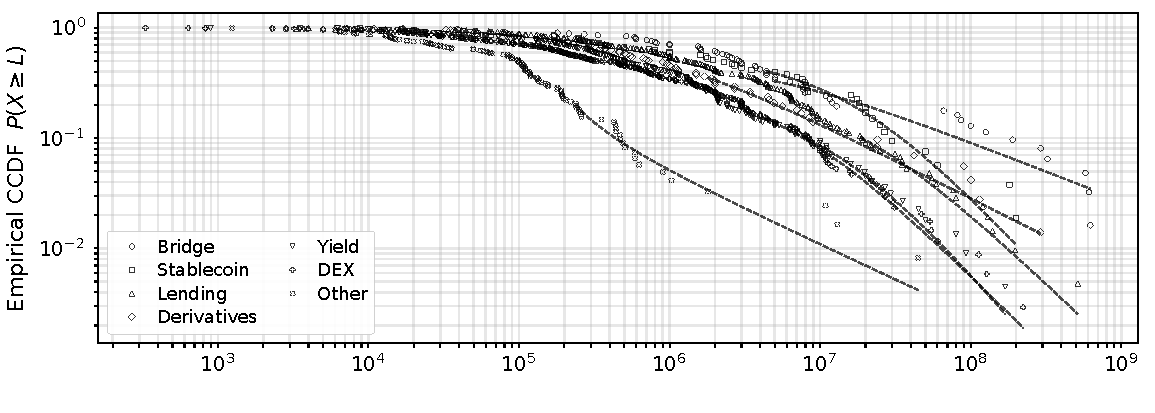
\includegraphics[width=\linewidth]{figures/ccdf_slide}\\[1.5mm]
  {\scriptsize Log-log CCDF, loss in USD along the horizontal axis, fitted
  POT-GPD dashed. Where $\hat\xi>1$ the fit turns up faster than the data at
  the top --- what the exposure cap addresses.\par}
\end{frame}

\begin{frame}{Frequency: events cluster, so Poisson understates}
  \begin{columns}[T]
    \begin{column}{0.55\textwidth}
      \footnotesize\setlength{\tabcolsep}{3pt}
      \begin{tabular}{l r r r r r r}
        \toprule
        Sector & $n$ & $\hat\mu_s$ & $\hat\lambda_s$ & $\hat\alpha_s$ & LR & $p$ \\
        \midrule
        Bridge      &  61 & 0.80 &  9.7 & 0.72 &  6.2 & 0.013 \\
        Lending     & 207 & 2.72 & 32.9 & 0.26 & 10.2 & 0.0014 \\
        Stablecoin  &  52 & 0.68 &  8.3 & 0.14 &  0.3 & 0.590 \\
        Derivatives &  71 & 0.93 & 11.3 & 0.41 &  3.7 & 0.054 \\
        Yield       & 222 & 2.92 & 35.3 & 0.60 & 42.3 & $7.7\!\times\!10^{-11}$ \\
        DEX         & 341 & 4.49 & 54.2 & 0.31 & 38.5 & $5.4\!\times\!10^{-10}$ \\
        Other       & 121 & 1.59 & 19.2 & 0.89 & 30.4 & $3.6\!\times\!10^{-8}$ \\
        \bottomrule
      \end{tabular}
    \end{column}
    \begin{column}{0.41\textwidth}
      \small
      \begin{itemize}
        \item Monthly counts are strongly over-dispersed: cross-sector
              dispersion index \hl{$D = 3.27$}.
        \item A likelihood-ratio test rejects Poisson at $p \le 0.02$ in
              \hl{five of seven} sectors.
        \item Annual event rates run from $8.3$/yr (Stablecoin) to
              $54.2$/yr (DEX).
      \end{itemize}
      \vskip 2mm
      Under Poisson the annual aggregate --- and its $\VaR_{99.9}$ --- would
      be understated.
    \end{column}
  \end{columns}
\end{frame}

\begin{frame}{The capital the tail implies}
  \begin{columns}[T]
    \begin{column}{0.55\textwidth}
      \footnotesize\setlength{\tabcolsep}{3pt}
      $\VaR_{99.9}$, \% of trailing-365d TVL
      \begin{tabular}{l r r r r l}
        \toprule
        Sector & $n$ & TVL (B) & $\VaR_{99.9}$ & $\VaR^{U}_{99.9}$ & IQR \\
        \midrule
        Bridge      &  61 & 49.1 & 32.5 & 67{,}326 & [25.5,\,40.8] \\
        Lending     & 207 & 66.8 & 18.0 & 22.3 & [3.2,\,18.9] \\
        Stablecoin  &  52 & 26.5$^\dagger$ & 16.1 & 16.1 & [3.1,\,30.1] \\
        Derivatives &  71 & 65.9 & 22.8 & 638.0 & [21.8,\,27.1] \\
        Yield       & 222 & 11.4 & 15.3 & 29.5 & [5.5,\,17.3] \\
        DEX         & 341 & 14.5 & 14.1 & 46.2 & [10.5,\,15.9] \\
        Other       & 121 & 18.2$^\ddagger$ & 27.5 & 285.9 & [4.8,\,27.7] \\
        \bottomrule
      \end{tabular}
      \vskip 1mm
      $^\dagger$circulating supply \quad $^\ddagger$residual TVL \quad
      $\VaR^{U}$: exposure cap removed
    \end{column}
    \begin{column}{0.41\textwidth}
      \small
      \begin{itemize}
        \item Core sectors need \hl{$14$--$18\%$ of TVL} --- far above the
              operational-risk capital banks hold.
        \item Bridge, Derivatives, Other look larger ($23$--$32\%$) but only
              because each event is \hl{capped at exposure}.
        \item Uncapped, $\hat\xi>1$ has no stable quantile: Bridge diverges to
              \hl{$673\times$ TVL}.
      \end{itemize}
    \end{column}
  \end{columns}
  \begin{pitfall}[The familiar pathology]
    The heaviest-tailed, most consequential sectors are exactly the ones the
    model cannot pin down unaided --- the instability that retired Basel's
    internal-model AMA in 2017.
  \end{pitfall}
\end{frame}

\begin{frame}{Sensitivity analysis}
  \begin{columns}[T]
    \begin{column}{0.48\textwidth}
      \textbf{Sensitivity to the largest events.}
      Dropping the single largest event moves $\hat\xi$ by $0.16$--$0.5$,
      most sharply in Lending ($0.75 \to 0.35$). Under any drop-top rule up to
      $0.5\%$, every sector keeps its \hl{below / above infinite-mean}
      character.
      \vskip 3mm
      \textbf{Sensitivity to the cap.}
      The cap binds: removing it lifts Lending $18 \to 22\%$, DEX
      $14 \to 46\%$, Yield $15 \to 30\%$. Only Stablecoin is
      cap-insensitive.
    \end{column}
    \begin{column}{0.48\textwidth}
      \textbf{Sensitivity to the confidence level.}
      At $99.5\%$ and $99\%$ the Lending requirement falls to $7\%$ and $5\%$
      of TVL, and buffered-venue coverage rises from $5\%$ to $18\%$ and
      $31\%$.
      \vskip 3mm
      \begin{takeaway}[Conclusions survive]
        Even at $99\%$, the buffers cover about a third of a requirement that
        is still an order of magnitude above bank operational-risk capital.
      \end{takeaway}
    \end{column}
  \end{columns}
\end{frame}

% =====================================================================
\section{Who bears it}
% =====================================================================

\begin{frame}{The protocol's response: capital buffers}
  Top-10 Lending venues by gross supplied TVL (DefiLlama, June~2026):
  \hl{four disclose an operational-risk reserve, six do not}.
  \vskip 2mm
  \begin{center}
    \small
    \begin{tabular}{l r r r r}
      \toprule
      Protocol & TVL (B) & Buffer (B) & $\E[S]$ (B) & $\VaR_{99.9}$ (B) \\
      \midrule
      Aave V3         & 11.85 & 0.36 & 0.08 ($475\%$) & 4.00 ($9\%$) \\
      SparkLend       &  3.41 & 0.08 & 0.02 ($390\%$) & 1.58 ($5\%$) \\
      Compound V3     &  1.04 & 0.04 & 0.01 ($700\%$) & 0.64 ($6\%$) \\
      Venus Core Pool &  0.98 & 0.01 & 0.01 ($187\%$) & 0.61 ($2\%$) \\
      \bottomrule
    \end{tabular}
  \end{center}
  \vskip 2mm
  Parentheses give the buffer's coverage of each. Average coverage of the
  modeled capital buffer: \hl{$\sim 5\%$}, a $95\%$ shortfall, from $2\%$
  (Venus) to $9\%$ (Aave~V3).
  \begin{takeaway}[The inadequacy is specific to the tail]
    All four buffers cover the pure premium at least once over
    ($187\%$--$700\%$). They are sized to an average year, not to a
    $1$-in-$1{,}000$ one.
  \end{takeaway}
\end{frame}

\begin{frame}{The depositor's response: the yield premium}
  Risk premium $=$ trailing-30d TVL-weighted stablecoin supply APY minus the
  $3.70\%$ 3-month T-bill.
  \vskip 1mm
  \begin{center}
    \footnotesize
    \begin{tabular}{l r r r r}
      \toprule
      Protocol & Total yield & Risk premium & $\E[S]$ & $\VaR_{99.9}$ \\
      \midrule
      \multicolumn{5}{l}{\emph{No buffer}} \\
      Morpho Blue   & 4.60\,\% & $+90$~bps  & $62$~bps ($144\%$)  & $3{,}905$~bps ($+2\%$) \\
      JustLend V1   & 3.42\,\% & $-28$~bps  & $60$~bps ($-47\%$)  & $4{,}785$~bps ($-1\%$) \\
      Kamino Lend   & 2.91\,\% & $-79$~bps  & $55$~bps ($-143\%$) & $6{,}169$~bps ($-1\%$) \\
      Jupiter Lend  & 4.64\,\% & $+94$~bps  & $55$~bps ($172\%$)  & $6{,}605$~bps ($+1\%$) \\
      Fluid Lending & 6.27\,\% & $+257$~bps & $52$~bps ($497\%$)  & $6{,}507$~bps ($+4\%$) \\
      Euler V2      & 3.59\,\% & $-11$~bps  & $47$~bps ($-23\%$)  & $8{,}131$~bps ($0\%$) \\
      \midrule
      \multicolumn{5}{l}{\emph{With buffer}} \\
      Aave V3         & 3.36\,\% & $-34$~bps  & $64$~bps ($-53\%$)  & $3{,}378$~bps ($-1\%$) \\
      SparkLend       & 2.84\,\% & $-86$~bps  & $60$~bps ($-143\%$) & $4{,}634$~bps ($-2\%$) \\
      Compound V3     & 2.85\,\% & $-85$~bps  & $55$~bps ($-155\%$) & $6{,}101$~bps ($-1\%$) \\
      Venus Core Pool & 2.09\,\% & $-161$~bps & $55$~bps ($-295\%$) & $6{,}226$~bps ($-3\%$) \\
      \bottomrule
    \end{tabular}
  \end{center}
  \small
  Unbuffered venues average \hl{$+54$~bps}: roughly their $55$-bps pure premium,
  but $1$--$4\%$ of the tail-risk premium --- and the buffers of the previous
  slide cover $\E[S]$ several times over while covering $5\%$ of
  $\VaR_{99.9}$. \hl{Protocol and depositor alike size their response to the
  loss of an average year, not to the extreme one.}
\end{frame}

\begin{frame}{Both margins together}
  Because buffer and premium substitute, an efficient market would trade one for
  the other --- buffered venues paying less. \hl{The data run in that direction.}
  \begin{itemize}
    \item Median premium: $-86$~bps with a buffer against $+39$~bps without ---
          a \hl{$125$-bps gap}. One-sided Mann--Whitney \hl{$p=0.01$}, and
          $p=0.03$ extending to all Lending venues with net TVL
          $\ge$ USD~$100$~m ($n=19$).
    \item Below that size the signal attenuates: posted yields are dominated by
          airdrops and incentives. The long-tail depositor is \hl{chasing
          incentives, not pricing risk}.
  \end{itemize}
  \begin{pitfall}[Right direction, wrong magnitude]
    The whole premium cross-section spans $418$~bps, while the tail asks for
    about $18\%$ of TVL. The market prices operational risk --- and still leaves
    the tail overwhelmingly unfunded on both margins.
  \end{pitfall}
\end{frame}

% =====================================================================
\section{What follows}
% =====================================================================

\begin{frame}{Who bears the shortfall, and what to do}
  \begin{columns}[T]
    \begin{column}{0.48\textwidth}
      \textbf{The shortfall is not evenly borne.}
      A professional participant can assess the tail, negotiate bilateral
      terms through governance, and size or exit the position. A \hl{retail
      depositor sees only the posted rate} and, lacking standardized
      disclosure, bears the unpriced tail disproportionately.
      \vskip 3mm
      Market discipline presumes the depositor \emph{can} price the risk. For
      the retail depositor that presumption fails twice over: the information
      is not disclosed, and pricing a heavy tail takes skills they do not have.
    \end{column}
    \begin{column}{0.48\textwidth}
      \textbf{So: disclosure, not capital mandates.}
      There is no clear path to imposing bank-style capital requirements on
      autonomous protocols. Three measures instead:
      \begin{enumerate}
        \item \hl{Standardized loss-and-yield disclosure} --- a Pillar~3
              analogue, per sector, alongside the posted yield.
        \item \hl{Buffer-and-tail disclosure} --- the buffer, the share of
              $\VaR_{99.9}$ it covers, the residual the depositor bears.
        \item \hl{Periodic recalibration} --- the tail is non-stationary.
      \end{enumerate}
      The duty can attach to whoever fronts access: front-ends, wallets,
      aggregators, custodial ``earn'' products.
    \end{column}
  \end{columns}
\end{frame}

\begin{frame}{Limitations and what I would fix next}
  \begin{columns}[T]
    \begin{column}{0.48\textwidth}
      \small
      \begin{itemize}
        \item \textbf{Incomplete data.} Publicly reported losses only; missing
              small and privately resolved incidents bias the body down,
              leave the tail intact.
        \item \textbf{Homogeneity.} One severity per sector, allocated by TVL
              share. A size covariate or a hierarchical model would refine it.
        \item \textbf{Recovery.} Figures are gross of funds returned, so the
              capital estimates are conservative.
      \end{itemize}
    \end{column}
    \begin{column}{0.48\textwidth}
      \small
      \begin{itemize}
        \item \textbf{Confounding.} Buffered venues are also the largest and
              oldest --- a descriptive association, not an identified buffer
              effect.
        \item \textbf{Premium identification.} The yield spread is
              reduced-form; it also reflects utilization and rate governance.
              A controlled panel regression is the natural extension.
        \item \textbf{Stationarity.} 2020--2026 fitted as one regime, though
              frequency has fallen and severity has concentrated.
      \end{itemize}
    \end{column}
  \end{columns}
\end{frame}

\begin{frame}{Conclusion}
  \begin{itemize}
    \item DeFi earn products carry a measurable operational-risk tail:
          USD~$9.45$~B over $1{,}075$ events, with four core sectors no
          heavier-tailed than banking and three past the infinite-mean
          boundary.
    \item Calibrated as a supervisor would, the Lending tail asks for
          \hl{$\sim 18\%$ of TVL} in capital.
    \item Against that benchmark, the four disclosed buffers cover
          \hl{$5\%$}, and unbuffered venues pay \hl{$+54$~bps} --- short of
          the tail by more than an order of magnitude.
    \item The two margins move together in the right direction, so the market
          does discriminate; it just does not price.
  \end{itemize}
  \begin{takeaway}[The recommendation]
    Not capital mandates on autonomous protocols, but \hl{disclosure} ---
    standardized loss, yield and buffer-coverage information, owed by the
    protocol or by whoever fronts access to it.
  \end{takeaway}
  \vskip 2mm
  \small
  Paper, data and code: \weblink{https://github.com/nbundi/pricing-the-defi-tail}{github.com/nbundi/pricing-the-defi-tail}
\end{frame}

\questionsslide
\closingslide

% =====================================================================
%  Backup slides
% =====================================================================
\appendix

\begin{frame}[noframenumbering]{Backup: threshold stability}
  \begin{center}
    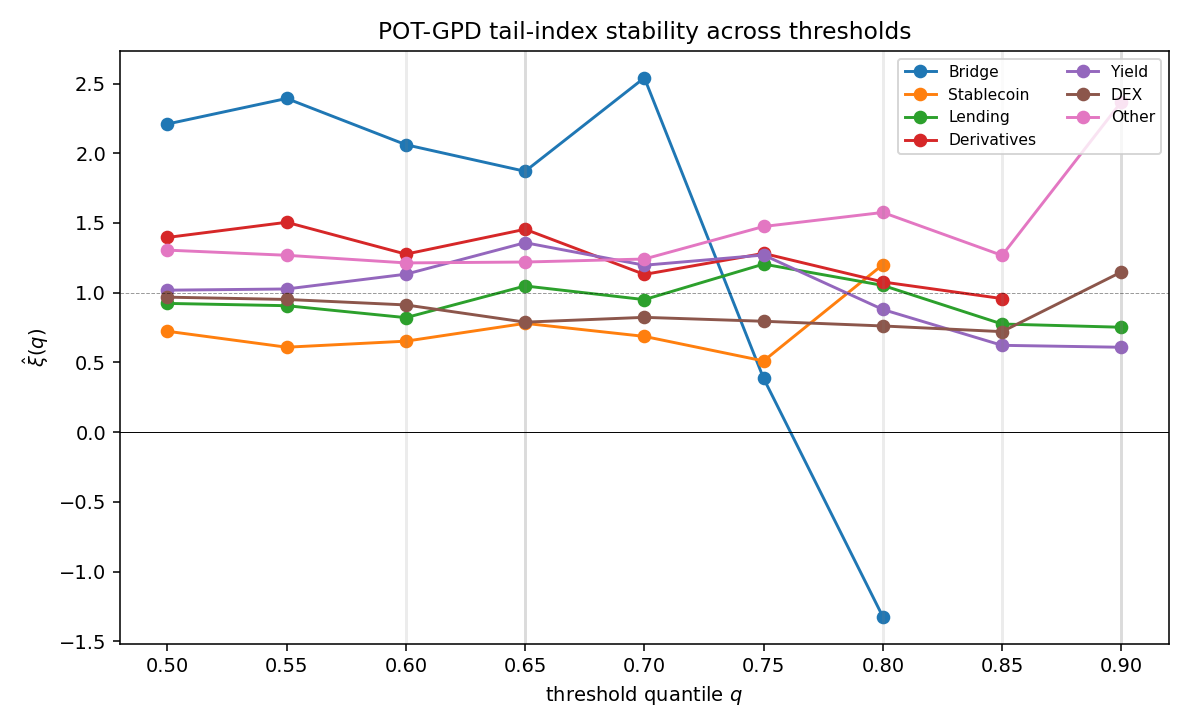
\includegraphics[width=0.62\linewidth]{figures/r5_xi_threshold_stability}
  \end{center}
  \small
  $\hat\xi$ against the threshold quantile. $q^*$ is the highest $q$ at which
  $\hat\xi(q)$ is stable to within $\tau=0.30$, subject to $n_u \ge 20$ and
  $n_u/n \ge 10\%$.
\end{frame}

\begin{frame}[noframenumbering]{Backup: event frequency over time}
  \begin{center}
    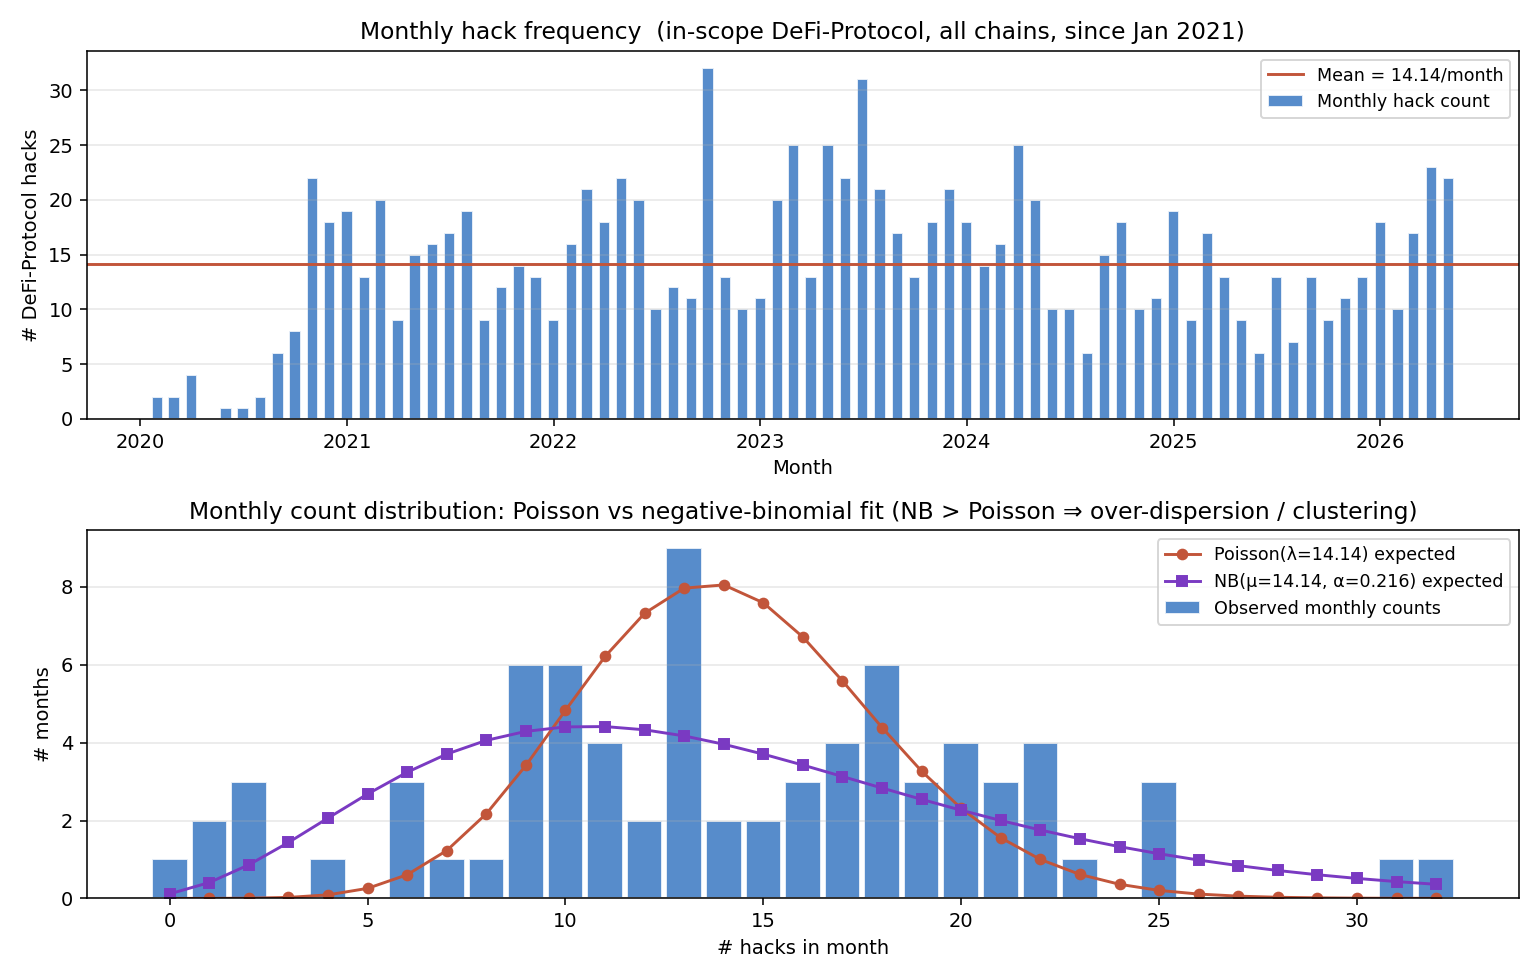
\includegraphics[width=0.62\linewidth]{figures/r6_monthly_counts}
  \end{center}
  \small
  Monthly event counts. Frequency has fallen from the early rugpull wave while
  severity has moved toward larger, concentrated targets --- the
  non-stationarity the stationary fit averages over.
\end{frame}

\begin{frame}[noframenumbering]{Backup: rolling intensity by sector}
  \begin{center}
    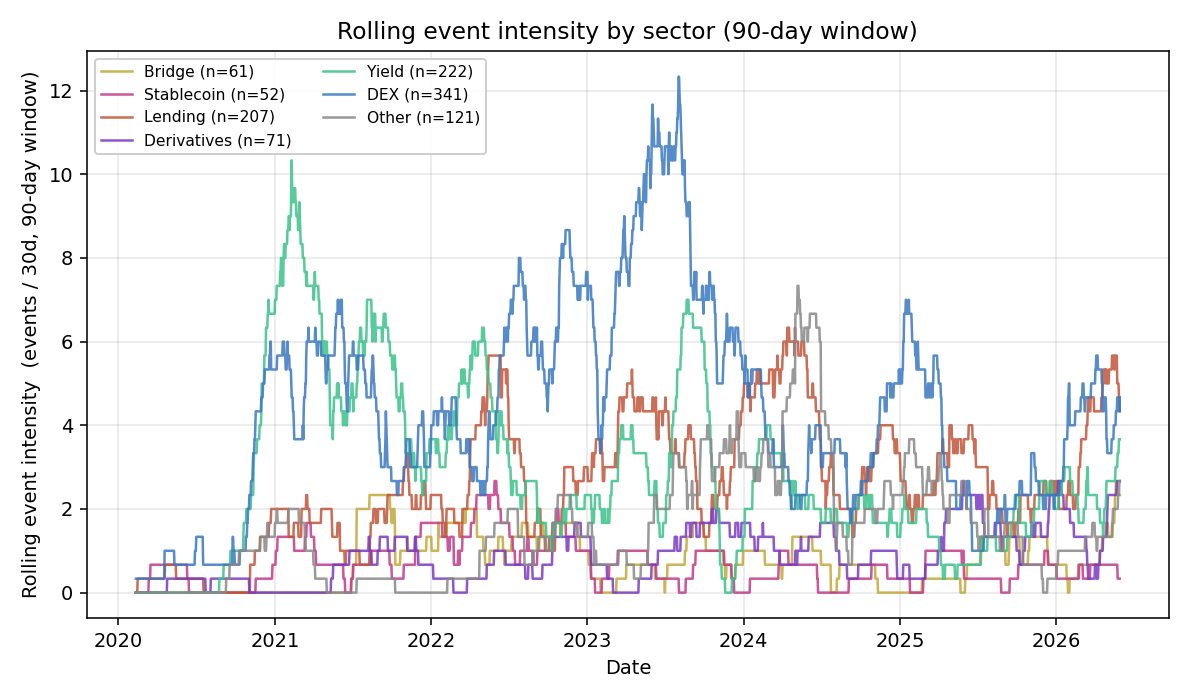
\includegraphics[width=0.66\linewidth]{figures/r0c_rolling_intensity_sector}
  \end{center}
\end{frame}

\end{document}
